\documentclass{article}
\usepackage{graphicx}
\usepackage{amsmath}
\renewcommand*\contentsname{Índice}

\begin{document}
\begin{titlepage}
\centering
    {
\includegraphics[width=0.5\textwidth]{logo}\par}
    \vspace{1cm}
    {\bfseries\LARGE Universidad Internacional de la Rioja \par}
    \vspace{1cm}
    {\scshape\Large Termodinámica \par}
    \vspace{3cm}
    {\scshape\Huge Laboratorio de termodinámica computacional \par}
    \vspace{3cm}
    \vfill
    {\Large Autor: \par}
    {\Large Jose R. Peña Seco \par}
    \vfill
    {\Large Enero 2024 \par}
\end{titlepage}

\tableofcontents
\pagebreak

\section{Introducción}


Los objetivos del laboratorio son realizar un estudio de los gases ideales. 
Para ello se realizarán una serie de mediciones sobre un simulador web de la presión de un gas ideal 
en función de la temperatura a volumen constante. Es decir, vamos a realizar una serie de procesos isostéricos.

\begin{figure}[h]
    \centering
    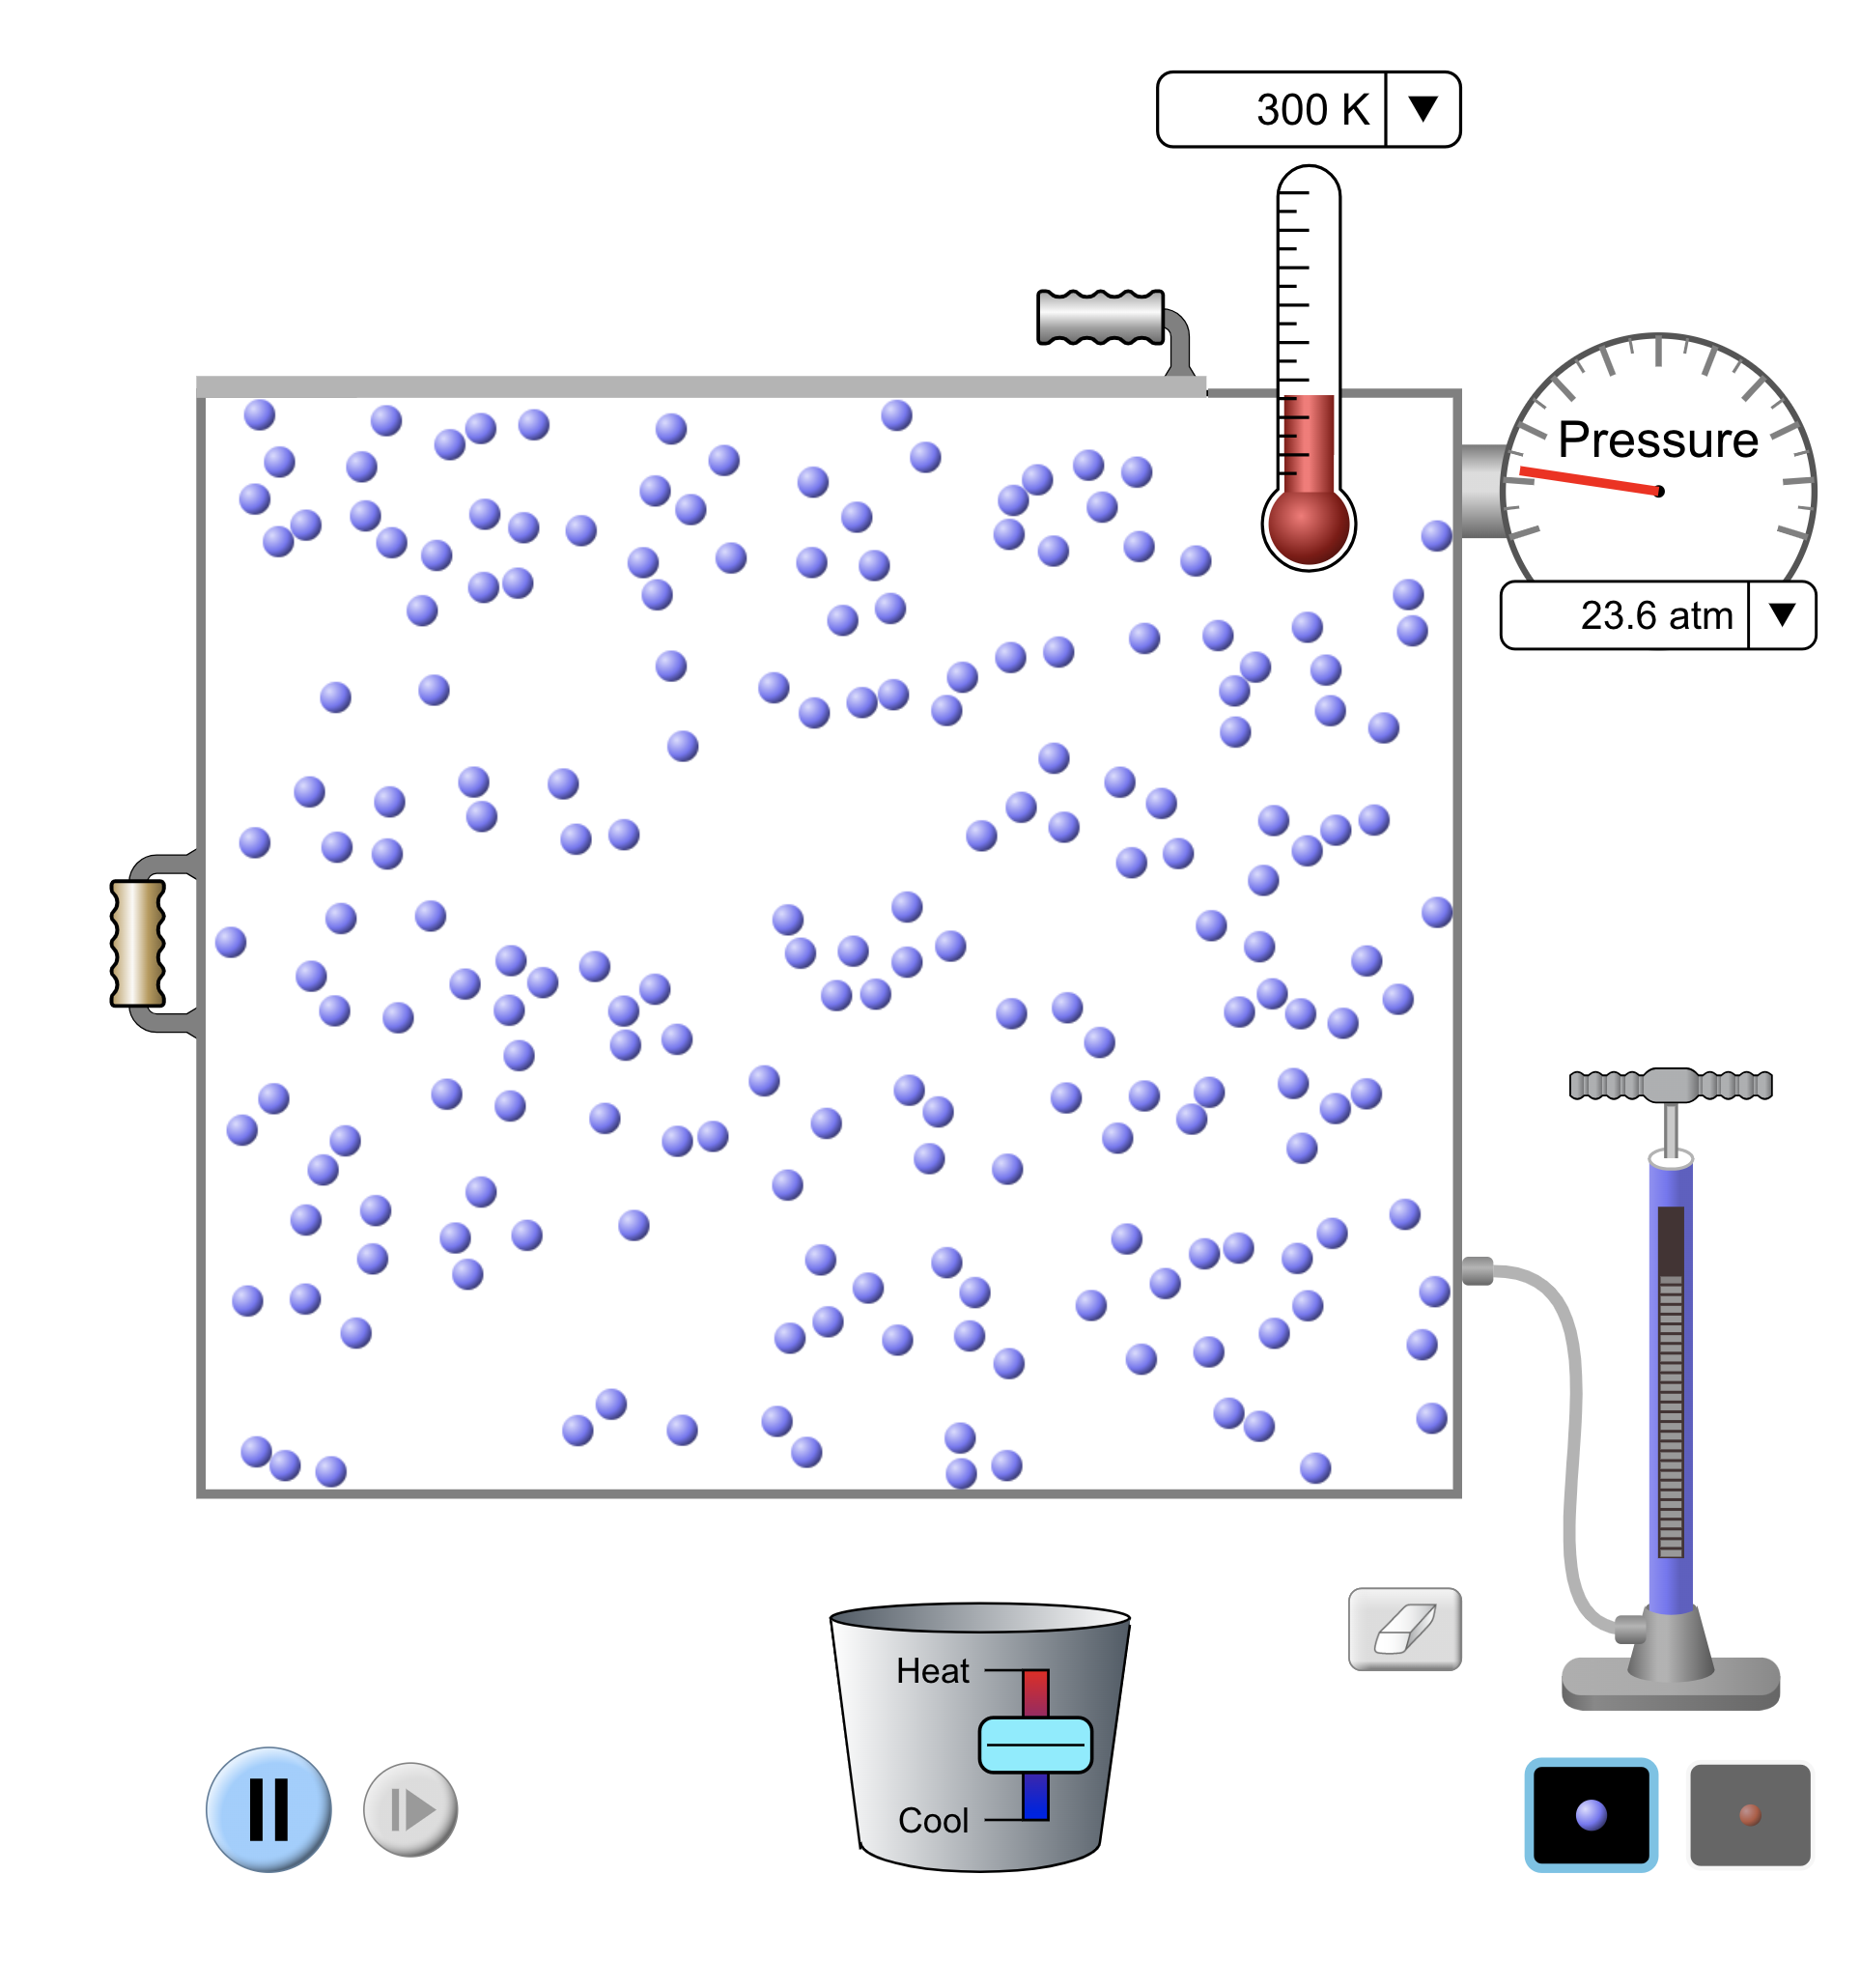
\includegraphics[width=0.6\textwidth]{lab2}
    \caption{Simulador web de la presión de un gas ideal en función de la temperatura a volumen constante}
\end{figure}

La imagen anterior muestra la herramienta de simulación utilizada para el estudio. 
La herramienta en cuestión es un laboratorio virtual que provee una representación visual 
interactiva de un sistema de partículas gaseosas, permitiendo al usuario manipular 
variables y observar los efectos resultantes.

En el centro del laboratorio podemos observar un recipiente que contiene 
partículas modeladas como esferas azules, las consideraremos partículas diatómicas, las cuales se desplazan 
libremente por el espacio confinado, simulando el movimiento térmico 
aleatorio de moléculas de gas. La temperatura del sistema está indicada por un
termómetro digital anexo que muestra un valor de 300 K, lo cual está en el rango 
de temperatura ambiente, y es un parámetro fundamental para entender la energía 
cinética promedio de las partículas. La presión ejercida por el gas se mide mediante 
un manómetro, que en esta instancia registra una presión de 23.5 atmósferas.

A lo largo del experimento iremos variando la temperatura del sistema y observaremos
como la presión del sistema varía en función de la misma. Iremos realizando las anotaciones
de los valores obtenidos en una tabla de datos que posteriormente utilizaremos para realizar
un análisis de los mismos.

\section{Parte I: Estudio de la ley de los gases ideales}
\subsection{Mediciones}

Las mediciones realizadas se muestran en la siguiente tabla:

\begin{center}
    \begin{tabular}{|c|c|c|}
        \hline
        Temperatura (C\textdegree) & Presión máxima (atm) & Presión mínima (atm) \\
        \hline
        27 & 23.7 & 23.0 \\
        \hline
        30 & 24 & 23.3 \\
        \hline
        33 & 24.2 & 23.5 \\
        \hline
        36 & 24.5 & 23.7 \\
        \hline
        39 & 24.7 & 24 \\
        \hline
        42 & 25 & 24.2 \\
        \hline
        45 & 25.3 & 24.4 \\
        \hline
        48 & 25.3 & 24.6 \\
        \hline
        51 & 25.6 & 24.9 \\
        \hline
        54 & 25.8 & 25.1 \\
        \hline
    \end{tabular}
\end{center}

El tratamiento de los datos se ha realizado en \textit{python} utilizando varias librerias conocidas 
como \textit{pandas} o \textit{numpy}. A continuación se muestra el código utilizado:
\begin{verbatim}
    import pandas as pd
    import numpy as np
    import matplotlib.pyplot as plt

    dataframe['p_avg'] = (dataframe['p_min'] + dataframe['p_max']) / 2
    dataframe['delta_temp'] = dataframe['temp'] - min(dataframe['temp'])
    dataframe['delta_p'] = dataframe['p_avg'] - min(dataframe['p_avg'])
\end{verbatim}

En primer lugar se ha calculado la media de las presiones máximas y mínimas para obtener una presión media.
A su vez se ha calculado el incremento de la temperatura y de la presión respecto a la primera medición.

Por último se ha empleado \textit{matplotlib} para generar una gráfica del incremento de la presión en función del incremento de la temperatura.
Finalmente creando un modelo de regresión lineal que se ajuste a estos datos. A continuación se muestra el código utilizado:

\begin{verbatim}
    def linear_regression(x, y):
    x_mean = np.mean(x)
    y_mean = np.mean(y)
    x_dev = x - x_mean
    y_dev = y - y_mean
    a = np.sum(x_dev * y_dev) / np.sum(x_dev * x_dev)
    b = y_mean - a * x_mean
    corrrelation_coefficient = np.sum(x_dev * y_dev) / np.sqrt(np.sum(x_dev * x_dev) * np.sum(y_dev * y_dev))
    print("slope: ", a)
    print("intercept: ", b)
    print("correlation coefficient: ", corrrelation_coefficient)
    return a, b, corrrelation_coefficient

    plt.plot(dataframe['delta_temp'], dataframe['delta_p'], 'o')
    plt.xlabel('delta_temp')
    plt.ylabel('delta_p')

    a, b, correlation_coefficient = linear_regression(dataframe['delta_temp'], dataframe['delta_p'])
    x = np.linspace(0, 30, 100)
    y = a * x + b
    plt.plot(x, y)

    plt.show()
\end{verbatim}

Finalmente se ha obtenido el siguiente gráfico:

\begin{figure}[h]
    \centering
    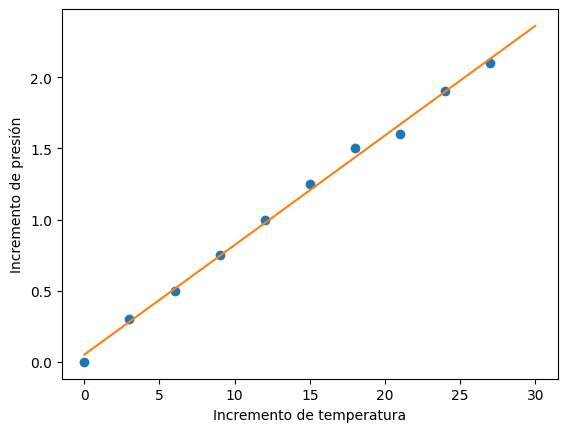
\includegraphics[width=0.8\textwidth]{chart1}
    \caption{plano de Clapeyron (T,P)}
\end{figure}

A su vez hemos obtenido los siguientes valores de a, b y el coeficiente de correlación:

\begin{verbatim}
    slope:  0.07696969696969702
    intercept:  0.05090909090909013
    correlation coefficient:  0.9982787839793615
\end{verbatim}

La pendiente (representada por 'a')
 indica la tasa de cambio en la presión con respecto a la temperatura. 
 En términos físicos, representa cómo la energía cinética promedio de las moléculas de gas 
 (y por lo tanto la presión) aumenta a medida que aumenta la temperatura. 
 Una mayor pendiente sugiere una mayor sensibilidad de la presión a los cambios 
 de temperatura para el gas específico estudiado.

Como podemos observar el coeficiente de correlación es muy cercano a 1, por lo que podemos afirmar que existe una relación lineal entre la presión y la temperatura como ya se ha visto en la teoría.
A su vez hay que apreciar que aunque el valor de la intersección no es cero, teoricamente debería de serlo. 
Esto se debe a que, según la ley de los gases ideales, si la temperatura es cero (en la escala Kelvin), la presión también debería ser cero.

Estos resultados pueden deberse a varios motivos
\begin{enumerate}
\item \textbf{Calibración del Instrumento:} Podría indicar un error de calibración en los instrumentos de medición. Por ejemplo, si el manómetro no está calibrado para mostrar cero a una presión atmosférica estándar, esto podría dar lugar a un intercepto no nulo.
\item \textbf{No Idealidad del Gas:} Si bien se están estudiando gases ideales, en la práctica, ningún gas es perfectamente ideal. Las desviaciones del comportamiento ideal (como las interacciones entre moléculas) podrían reflejarse en este intercepto no cero.
\item \textbf{Errores Experimentales:} El intercepto no cero también podría ser resultado de errores experimentales o limitaciones en la precisión de las mediciones.
\end{enumerate}

\subsection{Cálculo de moles}

Para calcular el número de moles de gas ideal que hay en el recipiente se puede utilizar la ecuación de estado de los gases ideales:


\begin{equation}
    PV = nRT
\end{equation}

\begin{equation}
    n = \frac{PV}{RT}
\end{equation}

A su vez tenemos la siguiente ecuación:

\begin{equation}
   \Delta T = a \cdot  \Delta P + b
\end{equation}

Conociendo que teóricamente b debería de ser cero, podemos igualar a a la siguiente expresión

\begin{equation}
   a = \frac{\Delta P }{\Delta T}
\end{equation}

Finalmente sustituyendo en la ecuación 2 tenemos:

\begin{equation}
    n = a \cdot \frac{V}{R}
\end{equation}

A continuación calculamos el volumen en litros asumiento que el recipiente es un cubo de 10 cm de lado:

\begin{equation}
    V = 10^3 cm^3 = 10^{-3} m^3 = 10^{-3} \cdot 10^3 dm^3 = 1 dm^3 = 1 L
\end{equation}

Y conociendo el valor de la constante de los gases ideales:

\begin{equation}
    R \approx 0,08206\; [L \cdot atm \cdot K^{-1} \cdot mol^{-1}]
\end{equation}

Finalmente obtenemos el número de moles:

\begin{equation}
    n \approx 0,076 \cdot \frac{1}{0,082} \approx 0,92 \; [mol]
\end{equation}

\subsection{Trabajo, calor y energía interna}

La expresión genérica en forma integral del trabajo realizado por un gas sería la siguiente

\begin{equation}
    W = \int_{V_0}^{V_1} p dV    
\end{equation}

En nuestro caso, como el volumen es constante \(dV = 0\), el trabajo realizado es cero.

\begin{equation}
    W = p \cdot \int_{V_0}^{V_1} dV = p \cdot (V_1 - V_0) = 0
\end{equation}

Por lo tanto 

\begin{equation}
    Q - W = \Delta U
\end{equation}

\begin{equation}
    Q = \Delta U
\end{equation}

Para conocer el valor de \(Q\) podemos utilizar la ecuación del calor molar que reza de la siguiente manera

\begin{equation}
    Q = n \cdot C_v \cdot \Delta T
\end{equation}

Sustituyendo en la expresión 12 tenemos que la variación de la energía interna es:

\begin{equation}
    \Delta U = n \cdot C_v \cdot \Delta T
\end{equation}

Finalmente teniendo en cuenta que el calor específico a volumen constante de un gas diatómico es:

\begin{equation}
    C_v = \frac{5}{2} \cdot R
\end{equation}

Sustituyendo en la expresión 14 tenemos que:

\begin{equation}
    \Delta U = n \cdot \frac{5}{2} \cdot R \cdot \Delta T
\end{equation}

Nuestros datos son los siguientes:

\begin{equation}
    \begin{split}
        & T_0 = 27 \textdegree C = 27 + 273 = 300 K  \\
        & T_1 = 54 \textdegree C = 54 + 273 = 327 K  \\
        & n = 0,92 \; [mol] \\
        & R \approx 8,314 \; [J \cdot K^{-1} \cdot mol^{-1}] \\
        & P_0 = 23,0 \; [atm] = 23,0 \cdot 101325 = 2330475 Pa \\
        & P_1 = 25,8 \; [atm] = 25,8 \cdot 101325 = 2619695 Pa \\
    \end{split}
\end{equation}

Sustituyendo en la expresión 15 tenemos que:

\begin{equation}
    \Delta U = 0,92 \cdot \frac{5}{2} \cdot 8,314 \cdot (327 - 300) \approx 516.29 \; [J]
\end{equation}

A continuación calcularemos la entalpía del sistema. Para ello utilizaremos la siguiente expresión:

\begin{equation}
    H = U + PV
\end{equation}

\begin{equation}
    \Delta H = \Delta U + P \cdot \Delta V
\end{equation}

Al no existir variación de volumen, la variación de la entalpía es igual a la variación de la energía interna:

\begin{equation}
    \Delta H = \Delta U = 516.29 \; [J]
\end{equation}

\section{Parte II: Estudio de un ciclo termodinámico}

A continuación realizaremos una serie de transformaciones termodinámicas para estudiar un ciclo termodinámico dentro del simulador.
Tomaremos los datos de cada una de las transformaciones y los anotaremos en una tabla para posteriormente realizar un análisis de los mismos.

Nuestro ciclo termodinámico constará de las siguientes transformaciones:
\begin{enumerate}
    \item \textbf{Transformación isobárica:} En esta transformación la presión se mantiene constante mientras que la temperatura varía.
    \item \textbf{Transformación isocórica:} En esta transformación el volumen se mantiene constante mientras que la temperatura varía.
    \item \textbf{Transformación isotérmica:} En esta transformación la temperatura se mantiene constante mientras que la presión varía.
    \item \textbf{Transformación isobárica:} En esta transformación la presión se mantiene constante mientras que la temperatura varía.
    \item \textbf{Transformación isocórica:} En esta transformación el volumen se mantiene constante mientras que la temperatura varía.
\end{enumerate}

\subsection{Mediciones}

Las mediciones correspondientes a cada una de las transformaciones son las siguientes

\begin{center}
    \begin{tabular}{|c|c|c|}
        \hline
        Temperatura (C\textdegree) & Lado (cm) & Presión media (atm) \\
        \hline
        27 & 10 & 23.45 \\
        \hline
        40 & 10.4 & 23.45 \\
        \hline
        60 & 10.4 & 23.85 \\
        \hline
        60 & 9 & 28.90 \\
        \hline
        96 & 10 & 28.90 \\
        \hline
        27 & 10 & 23.45 \\
        \hline
    \end{tabular}
\end{center}

Para realizar el análisis de los datos utilizaremos las mismas tecnologías que en el apartado anterior. 
Primero cargaremos el fichero \textit{csv} con los datos y posteriormente realizaremos los cálculos necesarios para obtener los datos que necesitamos.

\begin{verbatim}
    cicle = pd.read_csv('./ciclo.csv')
    cicle['p_avg'] = (cicle['p_min'] + cicle['p_max']) / 2
\end{verbatim}

Para crear las gráficas utilizaremos la librería \textit{matplotlib} teniendo el siguiente código:

Gráfica del plano de Clapeyron (V,P)

\begin{verbatim}
    plt.plot(cicle['lado']*(10**-3)**3, cicle['p_avg'], 'o')
    plt.xlabel('Volumen [L]')
    plt.ylabel('Presión [atm]')
    plt.plot(cicle['lado']*(10**-3)**3, cicle['p_avg'])
    plt.legend(['Datos experimentales', 'Ajuste lineal'])
    plt.show()
\end{verbatim}

Gráfica con el trabajo realizado

\begin{verbatim}
    plt.plot(cicle['lado']*(10**-3)**3, cicle['p_avg'], 'o')
    plt.xlabel('Volumen [L]')
    plt.ylabel('Presión [atm]')
    plt.plot(cicle['lado']*(10**-3)**3, cicle['p_avg'])
    plt.fill_between(cicle['lado']*(10**-3)**3, cicle['p_avg'], 25, alpha=0.5,)
    plt.legend(['Datos', 'Aproximación lineal', 'Trabajo'])
    plt.show()
\end{verbatim}

Quedando finalmente la gráfica:

\begin{figure}[h]
    \centering
    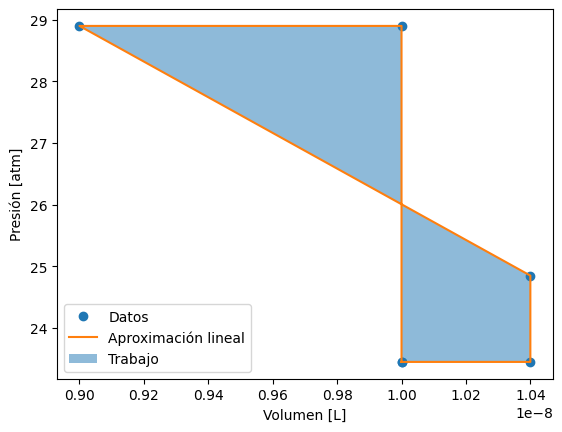
\includegraphics[width=0.8\textwidth]{cap2}
    \caption{plano de Clapeyron (V,P)}
\end{figure}

\subsection{Trabajo realizado}

\subsubsection{Transformación isobárica}

Comencemos por transformar las unidades de los datos obtenidos en la tabla a unidades del sistema internacional:

\begin{equation}
    \begin{split}
        & T_0 = 27 \textdegree C = 27 + 273 = 300 K  \\
        & T_1 = 40 \textdegree C = 40 + 273 = 313 K  \\
        & V_0 = 1000 \cdot 10^-6 = 10^{-3} \; [m^3]\\
        & V_1 = 1124,86 \; [cm^3] = 1.124 \cdot 10^{-3} \; [m^3] \\
        & P_0 = 23,45 \; [atm] = 23,45 \cdot 101325 = 2376071,25 \; [Pa] \\
    \end{split}
\end{equation}

A continuación calcularemos el trabajo realizado en esta transformación. Para ello utilizaremos la siguiente expresión:

\begin{equation}
    W = \int_{V_0}^{V_1} p dV
\end{equation}

Al ser la presión constante podemos sacarla fuera de la integral:

\begin{equation}
    W = p \cdot \int_{V_0}^{V_1} dV = p \cdot (V_1 - V_0)
\end{equation}

Finalmente obteniendo que el trabajo relizado es:

\begin{equation}
    W = 2376071,25\cdot ((1,1 \cdot 10^{-3}) - 10^{-3}) = 294.63
\end{equation}
Para realizar este trabajo el gas ha tenido que absorver calor. Para calcular la cantidad de calor que ha absorbido utilizaremos la siguiente expresión:

\begin{equation}
    Q = n \cdot C_p \cdot \Delta T
\end{equation}


\begin{equation}
    C_p = C_v + R
\end{equation}

\begin{equation}
    C_p = \frac{5}{2} \cdot R + R = \frac{7}{2} \cdot R
\end{equation}

\begin{equation}
    Q = n \cdot \frac{7}{2} \cdot R \cdot \Delta T
\end{equation}

\begin{equation}
    Q = 0,92 \cdot \frac{7}{2} \cdot 8,314 \cdot (313 - 300) \approx 348.02 \; [J]
\end{equation}

Finalmente calculamos la energia interna

\begin{equation}
    \Delta U = Q - W = 348.02 - 294.63 = 53.39 \; [J]
\end{equation}

Nuestra energia interna ha aumentado. Esto quiere decir que parte del calor absorbido se ha empleado para aumentar la energía interna del gas y
 el resto para realizar trabajo.

\subsubsection{Transformación isocórica}

Comencemos por transformar las unidades de los datos obtenidos en la tabla a unidades del sistema internacional:

\begin{equation}
    \begin{split}
        & T_0 = 40 \textdegree C = 40 + 273 = 313 K  \\
        & T_1 = 60 \textdegree C = 60 + 273 = 333 K  \\
        & V_0 = 1124 \; [cm^3] = 1.124 \cdot 10^{-3} \; [m^3]  \\
        & V_1 = 1124 \; [cm^3] = 1.124 \cdot 10^{-3} \; [m^3]  \\
        & P_0 = 23,45 \; [atm] = 23,45 \cdot 101325 = 2376231,25 \; [Pa] \\
        & P_1 = 23,85 \; [atm] = 23,85 \cdot 101325 = 2414237,25 \; [Pa] \\
    \end{split}
\end{equation}

A continuación calcularemos el trabajo realizado en esta transformación. Para ello utilizaremos la siguiente expresión:

\begin{equation}
    W = \int_{V_0}^{V_1} p dV
\end{equation}

Al ser el volumen constante podemos deducir que el trabajo realizado es cero:

\begin{equation}
    W = 0
\end{equation}

A su vez podemos calcular el calor absorbido por el gas para haber aumentado su temperatura utilizando la siguiente expresión:

\begin{equation}
    Q = n \cdot C_v \cdot \Delta T
\end{equation}

\begin{equation}
    Q = n \cdot \frac{5}{2} \cdot R \cdot \Delta T
\end{equation}

\begin{equation}
    Q = 0,92 \cdot \frac{5}{2} \cdot 8,314 \cdot (333 - 313) \approx 382.44 \; [J]
\end{equation}

Lógicamente al ser la energía interna una función de estado, y según la ley de joule \(U = f(T)\), 
la energía interna del gas ha tenido que aumentar.

Al no haberse realizado ningún trabajo, toda la energia calorifica 
se ha empleado para aumentar la energía interna del gas.

\begin{equation}
    \Delta U = Q = 382.44 \; [J]
\end{equation}

\subsubsection{Transformación isotérmica}

Comencemos por transformar las unidades de los datos obtenidos en la tabla a unidades del sistema internacional:

\begin{equation}
    \begin{split}
        & T_0 = 60 \textdegree C = 60 + 273 = 333 K  \\
        & T_1 = 60 \textdegree C = 60 + 273 = 333 K  \\
        & V_0 = 1124 \; [cm^3] = 1.123^{-3} \; [m^3] \\
        & V_1 = 729 \; [cm^3] = 0.729 \cdot 10^{-3} \; [m^3] \\
        & P_0 = 23,85 \; [atm] = 23,85 \cdot 101325 = 2416601,25 \; [Pa] \\
        & P_1 = 28,90 \; [atm] = 28,90 \cdot 101325 = 2416601,5 \; [Pa] \\
    \end{split}
\end{equation}

Para calcular el trabajo realizado en esta transformación utilizaremos la siguiente expresión:

\begin{equation}
    W = \int_{V_0}^{V_1} p dV
\end{equation}

Como la presión no es constante, no podemos sacarla fuera de la integral. Por lo tanto utilizaremos la expresión de los gases ideales para sustituir la presión:

\begin{equation}
    W = \int_{V_0}^{V_1} p dV = \int_{V_0}^{V_1} \frac{nRT}{V} dV = nRT \cdot \int_{V_0}^{V_1} \frac{1}{V} dV
\end{equation}

Finalmente obteniendo 

\begin{equation}
    W = nRT \cdot ln(\frac{V_1}{V_0})
\end{equation}

\begin{equation}
    W = 0,92 \cdot 8,314 \cdot 333 \cdot ln(\frac{0,729}{1,123}) \approx - 1100.55 \; [J]
\end{equation}

Es lógico que el trabajo sea negativo puesto que para comprimirse se ha tenido que realizar un trabajo exterior sobre el gas.
A su vez la energia interna no cambia ya que la temperatura se mantiene constante.

Podemos asumir que la cantidad de calor absorbido es igual al trabajo realizado debido a
que el gas no ha variado su temperatura:

El signo significa que el cuerpo ha liberado calor, esto tiene sentido ya que ha aumentado
su presión, y este cambio de presión mantiene la temperatura constante.

\begin{equation}
    Q = -1100.55 \; [J]
\end{equation}

Por lo tanto la variación de la energía interna es:

\begin{equation}
    \Delta U = 0
\end{equation}

\subsubsection{Transformación isobárica}

Comencemos por transformar las unidades de los datos obtenidos en la tabla a unidades del sistema internacional:

\begin{equation}
    \begin{split}
        & T_0 = 60 \textdegree C = 60 + 273 = 333 K  \\
        & T_1 = 96 \textdegree C = 96 + 273 = 369 K  \\
        & V_0 = 729 \; [cm^3] = 0.729 \cdot 10^{-3} \; \\
        & V_1 = 1000 \; [cm^3] = 10^{-3} \; \\
        & P_0 = 28,90 \; [atm] = 28,90 \cdot 101325 = 2928292,5 \; [Pa] \\
        & P_1 = 28,90 \; [atm] = 28,90 \cdot 101325 = 2928292,5 \; [Pa] \\
    \end{split}
\end{equation}

Para ello podemos usar la ecuación obtenida en la transformación isobárica:

\begin{equation}
    W = p \cdot (V_1 - V_0)
\end{equation}

\begin{equation}
    W = 2928292,5 \cdot (1 \cdot 10^{-3} - 0,729 \cdot 10^{-3}) = 793.56 \; [J]
\end{equation}

A su vez ha absorvido calor para aumentar su temperatura. Para calcular la cantidad de calor que ha absorbido utilizaremos la siguiente expresión:

\begin{equation}
    Q = n \cdot C_p \cdot \Delta T
\end{equation}

\begin{equation}
    Q = n \cdot \frac{7}{2} \cdot R \cdot \Delta T
\end{equation}

\begin{equation}
    Q = 0,92 \cdot \frac{7}{2} \cdot 8,314 \cdot (369 - 333) \approx 963.75 \; [J]
\end{equation}


Por lo tanto la variación de la energía interna es:

\begin{equation}
    \Delta U = Q - W = 963.75 - 793.56 = 170.19 \; [J]
\end{equation}

Como es obvio es positiva ya que el gas ha usado parte del calor absorbido para aumentar su energía interna y el resto para realizar trabajo.

\subsubsection{Transformación isocórica}

Comencemos por transformar las unidades de los datos obtenidos en la tabla a unidades del sistema internacional:

\begin{equation}
    \begin{split}
        & T_0 = 96 \textdegree C = 96 + 273 = 369 K  \\
        & T_1 = 27 \textdegree C = 27 + 273 = 300 K  \\
        & V_0 = 1000 \; [cm^3] = 10^{-3} \; [m^3] = 10^{-3} \cdot 10^3 \; [dm^3] = 1 \; [dm^3] = 1 \; [L] \\
        & V_1 = 1000 \; [cm^3] = 10^{-3} \; [m^3] = 10^{-3} \cdot 10^3 \; [dm^3] = 1 \; [dm^3] = 1 \; [L] \\
        & P_0 = 28,90 \; [atm] = 28,90 \cdot 101325 = 2927227,5 \; [Pa] \\
        & P_1 = 23,45 \; [atm] = 23,45 \cdot 101325 = 2376231,25 \; [Pa] \\
    \end{split}
\end{equation}

De nuevo el trabajo realizado es cero ya que el volumen es constante.

\[
    W = 0
\]

Sin embargo el gas ha cedido calor para disminuir su temperatura. Para calcular la cantidad de calor que ha cedido utilizaremos la siguiente expresión:

\begin{equation}
    Q = n \cdot C_v \cdot \Delta T
\end{equation}

\begin{equation}
    Q = n \cdot \frac{5}{2} \cdot R \cdot \Delta T
\end{equation}

\begin{equation}
    Q = 0,92 \cdot \frac{5}{2} \cdot 8,314 \cdot (300 - 369) \approx - 1319.43 \; [J]
\end{equation}

\subsubsection{Trabajo total y calor total}

Finalmente el trabajo total realizado es la suma de los trabajos realizados en cada una de las transformaciones:

\begin{equation}
    W_{total} = 294,63 + 0 + (-1100,55) + 793,56 + 0 = -12,36 \; [J]
\end{equation}

Y el calor total absorvido

\begin{equation}
    Q_{total} = 348,02 + 382,44 ' 1100,55 + 963,75 + (-1319,43) = - 725,77 \; [J]
\end{equation}

Por lo tanto la variación de la energía interna es:

\begin{equation}
    \Delta U = Q_{total} - W_{total} = -725,77 + 12,36 = -713,41 \; [J]
\end{equation}

Como podemos ver el trabajo total es negativo puesto que este ha sido realizado sobre el sistema y el calor total es negativo puesto que el sistema ha cedido calor.
Es por ello que la energía interna ha disminuido.

\subsection{Calculo del trabajo gráfico}

Para ello hemos utilizado \textit{python}. La librería \textit{numpy}
tiene una función llamada \textit{trapz} que nos permite calcular el área bajo
 la curva utilizando el método de integración trapezoidal.

\begin{verbatim}
    cicle['p_pascal'] = cicle['p_avg'] * 101325
    cicle['volumen_m3'] = (cicle['lado'] * (10**-2))**3

    # Extract the volume and pressure values as numpy arrays for trapezoidal integration
    volumes = cicle['volumen_m3'].to_numpy()
    pressures = cicle['p_pascal'].to_numpy()


    # Calculate the area under the curve using trapezoidal integration
    area = np.trapz(pressures, volumes)
\end{verbatim}

El resultado final calculado es el siguiente:

\begin{verbatim}
    area = 12.27205843500019
\end{verbatim}

El resultado es bastante similar al obtenido en el cálculo analítico. Sin embargo difiere un poco seguramente
por la aproximación lineal que hemos realizado. A su vez comentar que el signo de un area al siempre ser positivo no nos aporta información a cerca 
si el trabao ha sido realizado sobre el exterior hacia el sistema o del sistema sobre el exterior.

\subsection{Eficiencia del ciclo}

Para calcular la eficiencia del ciclo utilizaremos la siguiente expresión:

\begin{equation}
    \eta = \frac{W_{total}}{Q_{total}} = \frac{-12,36}{-725,77} = 0,017
\end{equation}

Finalmente comparamos con el ciclo de Carnot:

\begin{equation}
    \eta_{carnot} = 1 - \frac{T_{min}}{T_{max}} = 1 - \frac{300}{369} = 0,19
\end{equation}


Como se puede observar la eficiencia del ciclo es bastante inferior a la del ciclo de Carnot como es lógico puesto que 
este ciclo es el mas eficiente posible.

\pagebreak

\section{Enlaces y documentación}
\begin{enumerate}
    \item Repositorio github: dentro de este repositorio se encuentra el código utilizado para realizar los cálculos y las gráficas. Enlace: https://github.com/josericardopenase/lab-termodinamica-computacional.git
\end{enumerate}

\end{document}